\chapter{Instruments}
\label{chapter:instruments}

In the following chapters I present data and results from a variety of configurations of two massively redundant low frequency interferometers, PAPER and HERA. In this Chapter I describe these instruments (Section~\ref{sec:used_in_this_work}), along with other current and future low frequency interferometers contributing to EoR science (Section~\ref{sec:not_used_in_this_work}).

\section{Instruments used in this work}
\label{sec:used_in_this_work}

The vision of Hydrogen Epoch of Reionization Arrays was first laid out in the \cite{HERAWhitePaper} White Paper. That work proposed three consecutive efforts, improving upon their predecessors, to construct low frequency interferometers capable of detecting the EoR. While the physical feeds and elements of low frequency interferometers were relatively simple to construct, signal processing, calibration and imaging required new hardware and software to be invented. A research community of observational cosmologists interested in cosmological {\sc hi} had to be nurtured.

The first of the three stages of Reionization Arrays was a parallel effort. The Precision Array for Probing the Epoch of Reionization (PAPER; Section~\ref{subsec:paper_instrument}) and the Murchinson Widefield Array (MWA; Section~\ref{subsec:mwa_instrument}) investigated separate approaches to\footnote{Among other things; see Section III B of \citet{HERAWhitePaper} for an enumerated list.} antenna design, array layout and calibration techniques, with the objective of setting upper limits on and perhaps detecting the power spectrum of the EoR.

The second stage of the Reionization Arrays brought together the teams from the first stage to design and construct a new interferometer based on the lessons learned from PAPER and the MWA. This new instrument, named \textit{the} Hydrogen Epoch of Reionization Array (HERA; Section~\ref{subsec:hera_instrument}) is currently under construction with a build-out schedule that brings new antennas online as they are commissioned. HERA's objective is not only the detection of the EoR power spectrum, but its characterization at very high signal-to-noise. Attempts at low-fidelity imaging of ionized bubbles will be made.

The nature of the third stage is, at the time of writing, somewhat undetermined and contingent on the next decade of funding for low frequency radio astronomy. In the vision of \cite{HERAWhitePaper}, its objective will be to image structure evolution throughout the EoR.

\subsection{The Donald C. Backer Precision Array for Probing the Epoch of Reionization (PAPER)}
\label{subsec:paper_instrument}

Much of this thesis presents data from PAPER. PAPER was planned, like HERA, as a staged build-out to larger and larger arrays. In each build-out the correlator was replaced, and (nominally) identical antennae and signal chains were added to the existing array. The first iterations of PAPER consisted of 8 dipole antennae in Green Bank, West Virginia and 4 in Western Australia \citep{Parsons.10}. While the Australian site had a far better observing environment in terms of human-generated radio interference, the site in the USA was easier for the team to design and test on. Green Bank was intended as a test site -- brighter foregrounds in the Northern Hemisphere and an unprotected low frequency band inhibited the science goals of the experiment. Nonetheless, the array in Green Bank was build-up to 32 antennae and reconfigured from a more traditional imaging configuration to a redundant grid, in order to experiment with redundant calibration and increased sensitivity to discrete Fourier modes \citep{Parsons.12b, Pober.12}. Simultaneously, the PAPER-32 array and correlator were constructed in the Karoo Radio Quiet Zone (KRQZ) in South Africa.

\subsubsection{The PAPER signal chain}

The PAPER signal chain changed little throughout the PAPER build-outs in South Africa, and it remained in operation for the HERA-19 Commissioning Array out to HERA-127. HERA elements are actually PAPER feeds, turned upside-down and suspended over a 14\,m dish. This heritage was important to understand when interpreting PAPER or HERA data. We briefly describe the PAPER signal chain below. For a more thorough description, refer to \cite{Parsons.10}.

Radio waves were incident upon, and induced a voltage in, a dual-polarization PAPER feed. The feed was a sleeved copper dipole protected by a wire-mesh groundscreen. The sleeve broadened the frequency response of the dipole element, and the groundscreen was used to increase sensitivity to emission from zenith (see Figure~\ref{fig:instruments_PAPER_element} for a photograph).

\begin{figure}
\centering
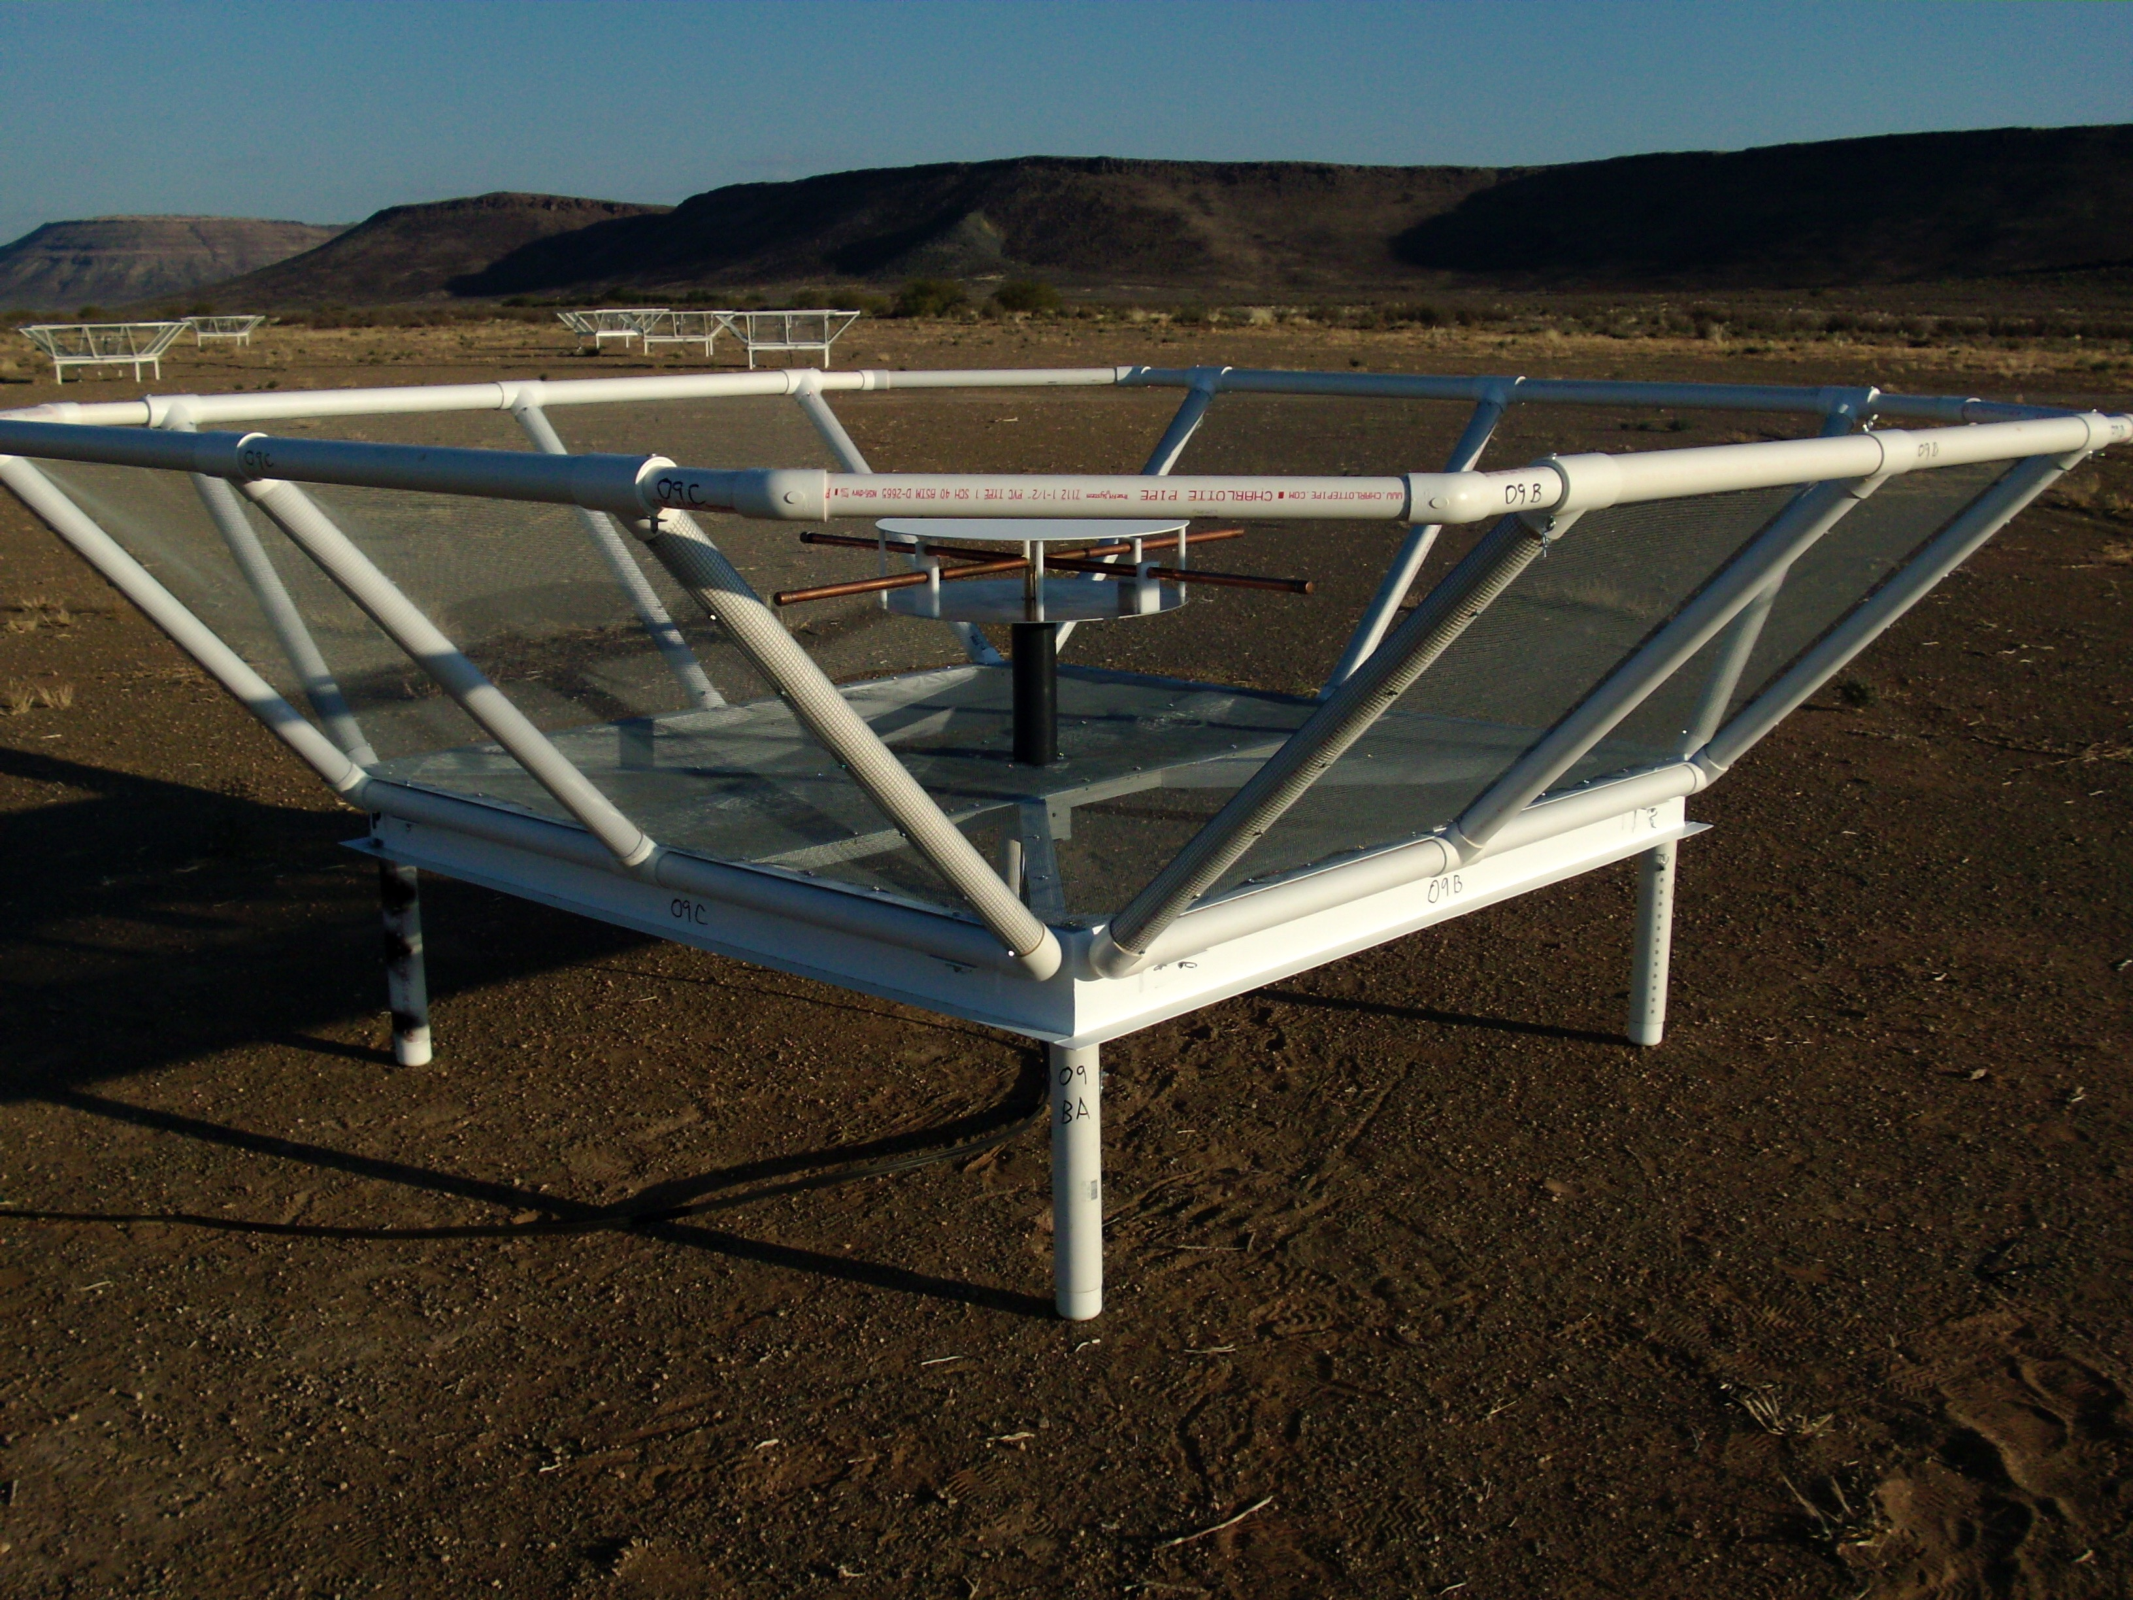
\includegraphics[width=0.9\textwidth]{chapters/instruments/figures/PAPER_dipole.pdf}
\caption{An image of a PAPER dipole element with its groundscreen.}
\label{fig:instruments_PAPER_element}
\end{figure}


Electronics next to the dipole element amplified the voltage by a factor of $10^6$, which then propagated down a 150 foot 75\,$\Omega$ coaxial cable. All cables were of the same length to minimize the amount of extra calibration required per feed, and were above-ground. These cables ran to 8 ``receiverators''; RFI-shielded mini-fridges which contained amplifiers which re-amplified the voltage signals by a factor of $10^4$  (to correct for signal loss along the 150\,ft coaxial cables) and applied an analog bandpass filter. The filter was designed to have a smooth frequency response which was relatively flat between 120 and 180 MHz \citep[e.g.][]{MooreThesis}.

More 50 foot, 75\,$\Omega$ foot coaxial cables ran from these to an RFI-shielded enclosure for further processing. For PAPER and the HERA-19 commissioning array, this enclosure was a specialized shipping container next to the array. For future HERA build-outs, processing will occur in the Karro Array Processing Building (KAPB) and the receiverator architecture will be replaced with underground ``nodes'' (see \citet{deBoer.17} for more detail).

The filtered analog signal was then digitized with a sampling rate of 100 MHz and passed through an F-engine which Fourier transforms the signal using a 4-tap polyphase filter bank (which allowed for a smooth frequency and Fourier-space response; \citet{PricePFB}). The integration time of each Fourier transform was 10\,s. The Fourier transformed signals were distributed over a 10 Gigabit Ethernet switch to the X-engine \citep{Parsons.08}, which cross-multiplied all signals with each other to form visibilities, storing them in {\sc miriad} files.

A summary of the system described above is shown in Figure~\ref{fig:instruments_PAPER_Signal_Chain}.

\begin{figure}
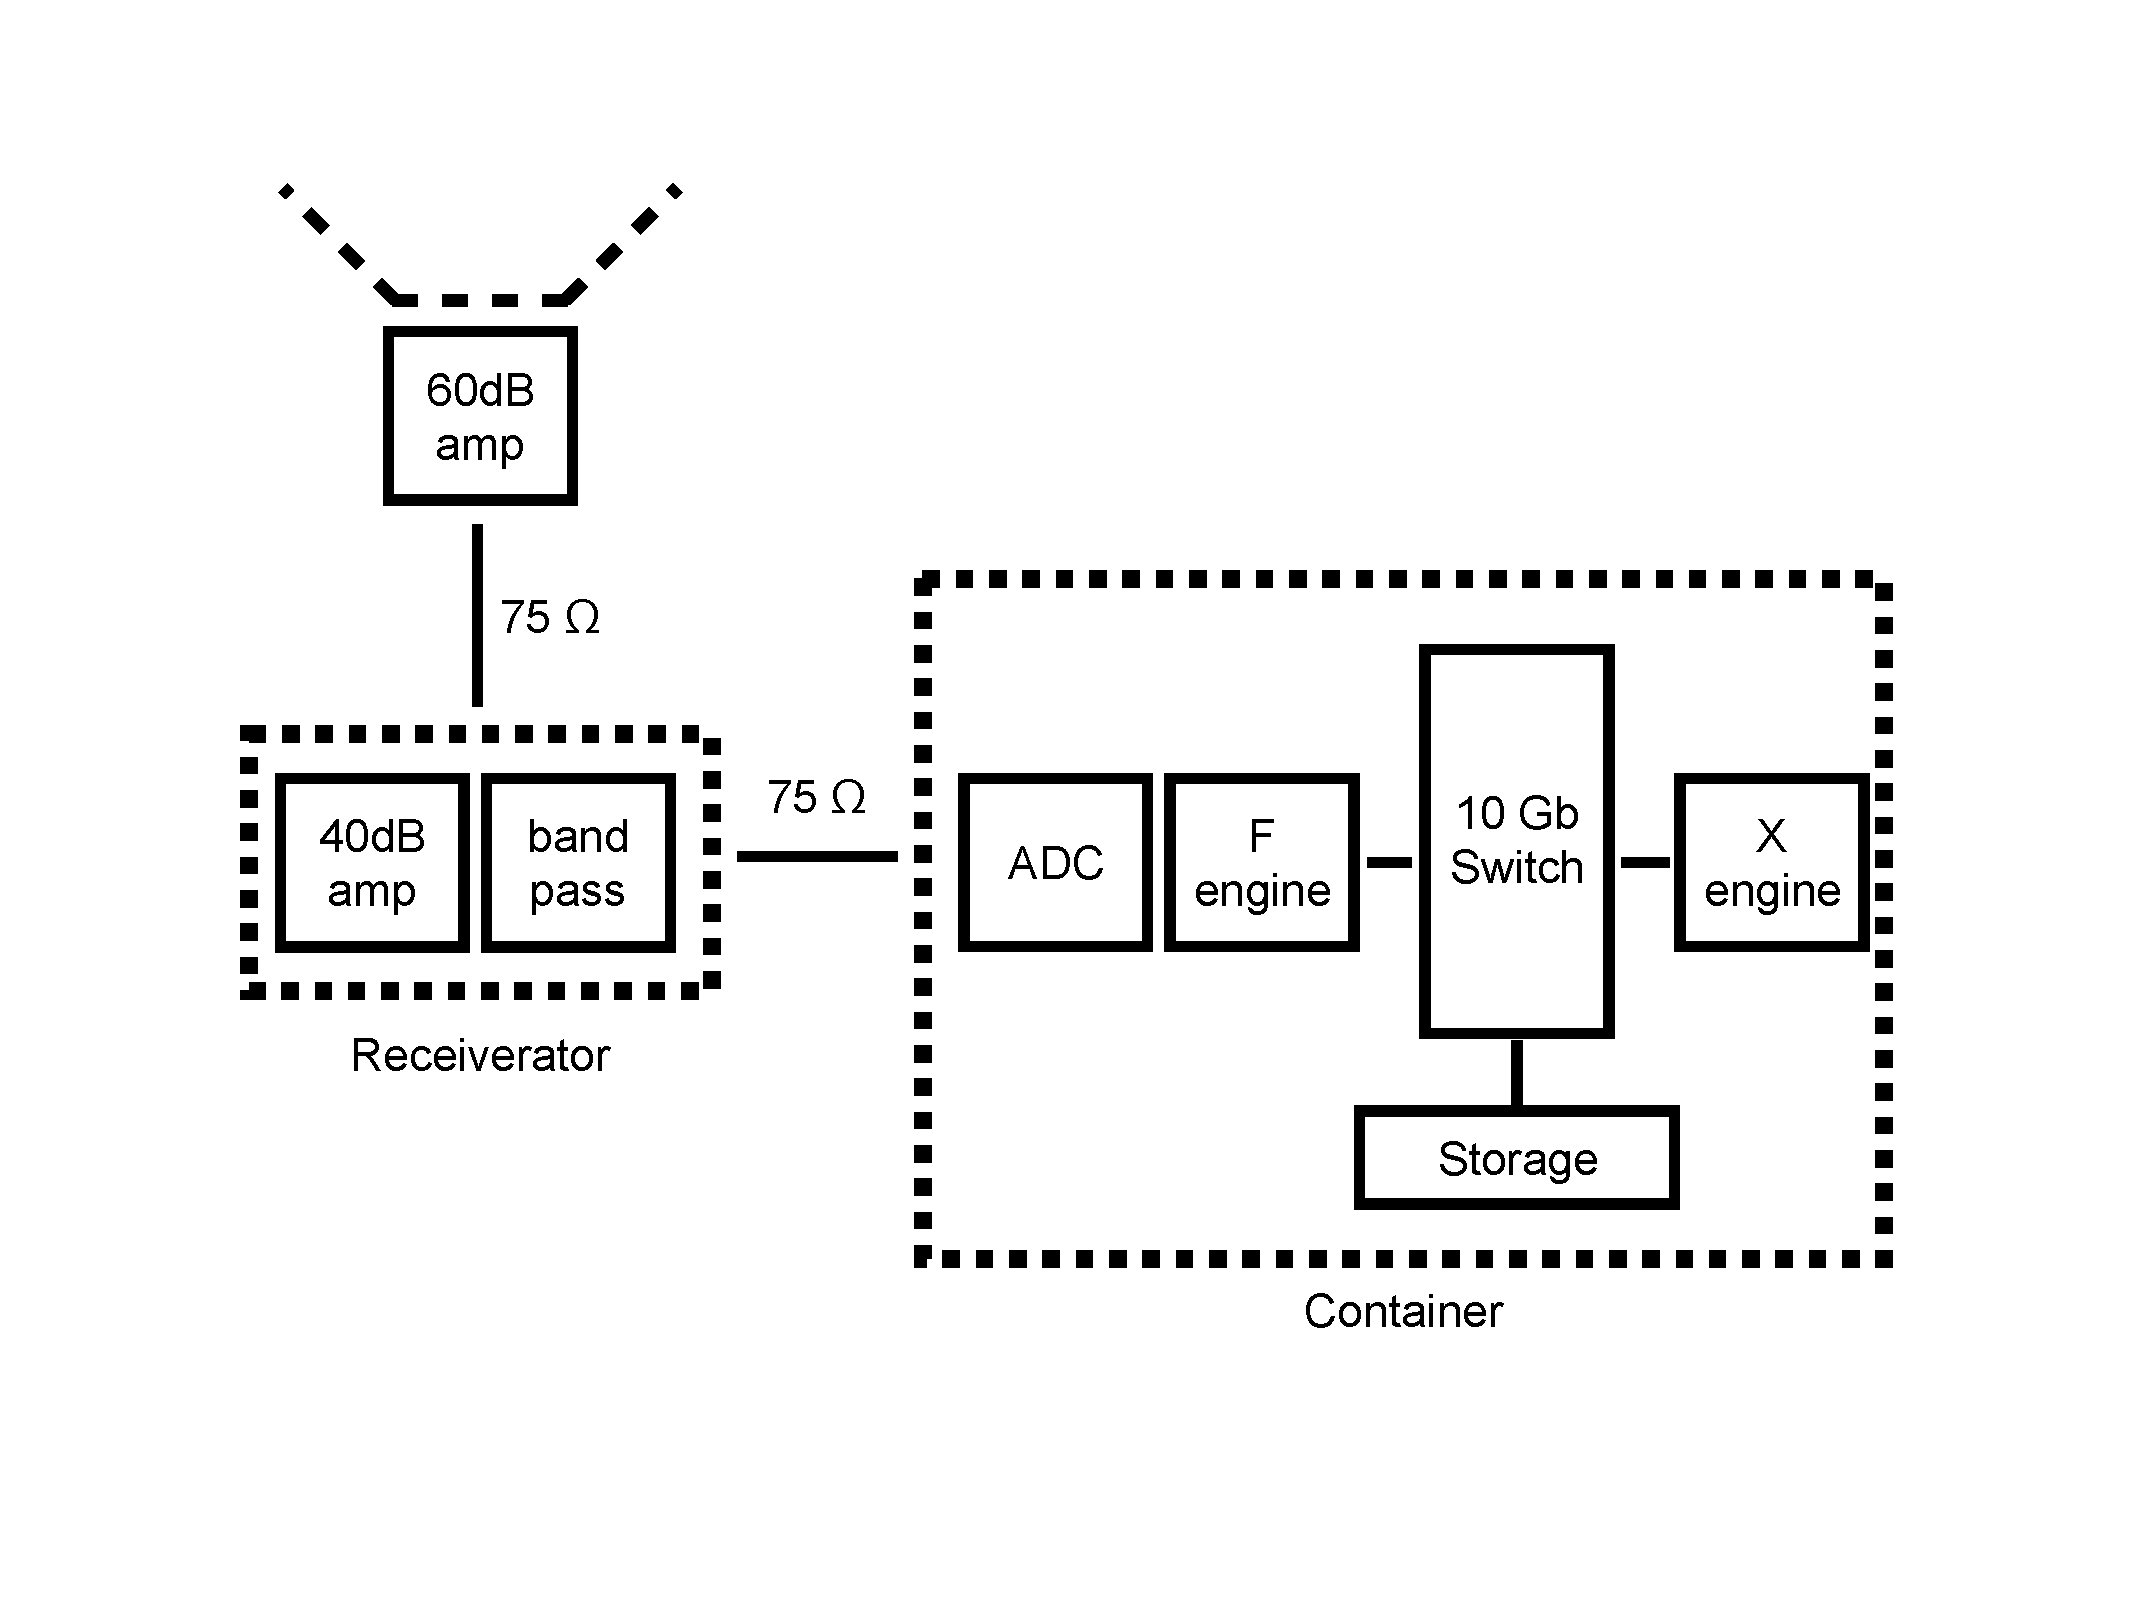
\includegraphics[width=0.9\textwidth]{chapters/instruments/figures/PAPER_system_diagram.pdf}
\caption{A diagram of the PAPER-128 signal chain. Square-dotted lines indicate RFI-shielding.}
\label{fig:instruments_PAPER_Signal_Chain}
\end{figure}

\subsubsection{PAPER-32}

The PAPER-32 array in South Africa used a highly redundant configuration in order to take the measurements resulting in, at the time, the strongest upper limits on the EoR power spectrum \citep[][sections of \citealt{Moore.17} are presented in Chapter~\ref{chapter:ionosphere}]{Parsons.14, Jacobs.15, Moore.17}. The array was in redundant configuration from December 2011 to February 2012. For three nights in September 2011, the 32 elements were reconfigured into an polarized imaging configuration. The results from this deployment were used to make the first 2D power spectra of polarization, presented in \cite{Kohn.16} and in Chapter~\ref{chapter:eor_window_paper32img}. For images and a brief description, see Figure~\ref{fig:instruments_psa32layout}.

\begin{figure}
\centering
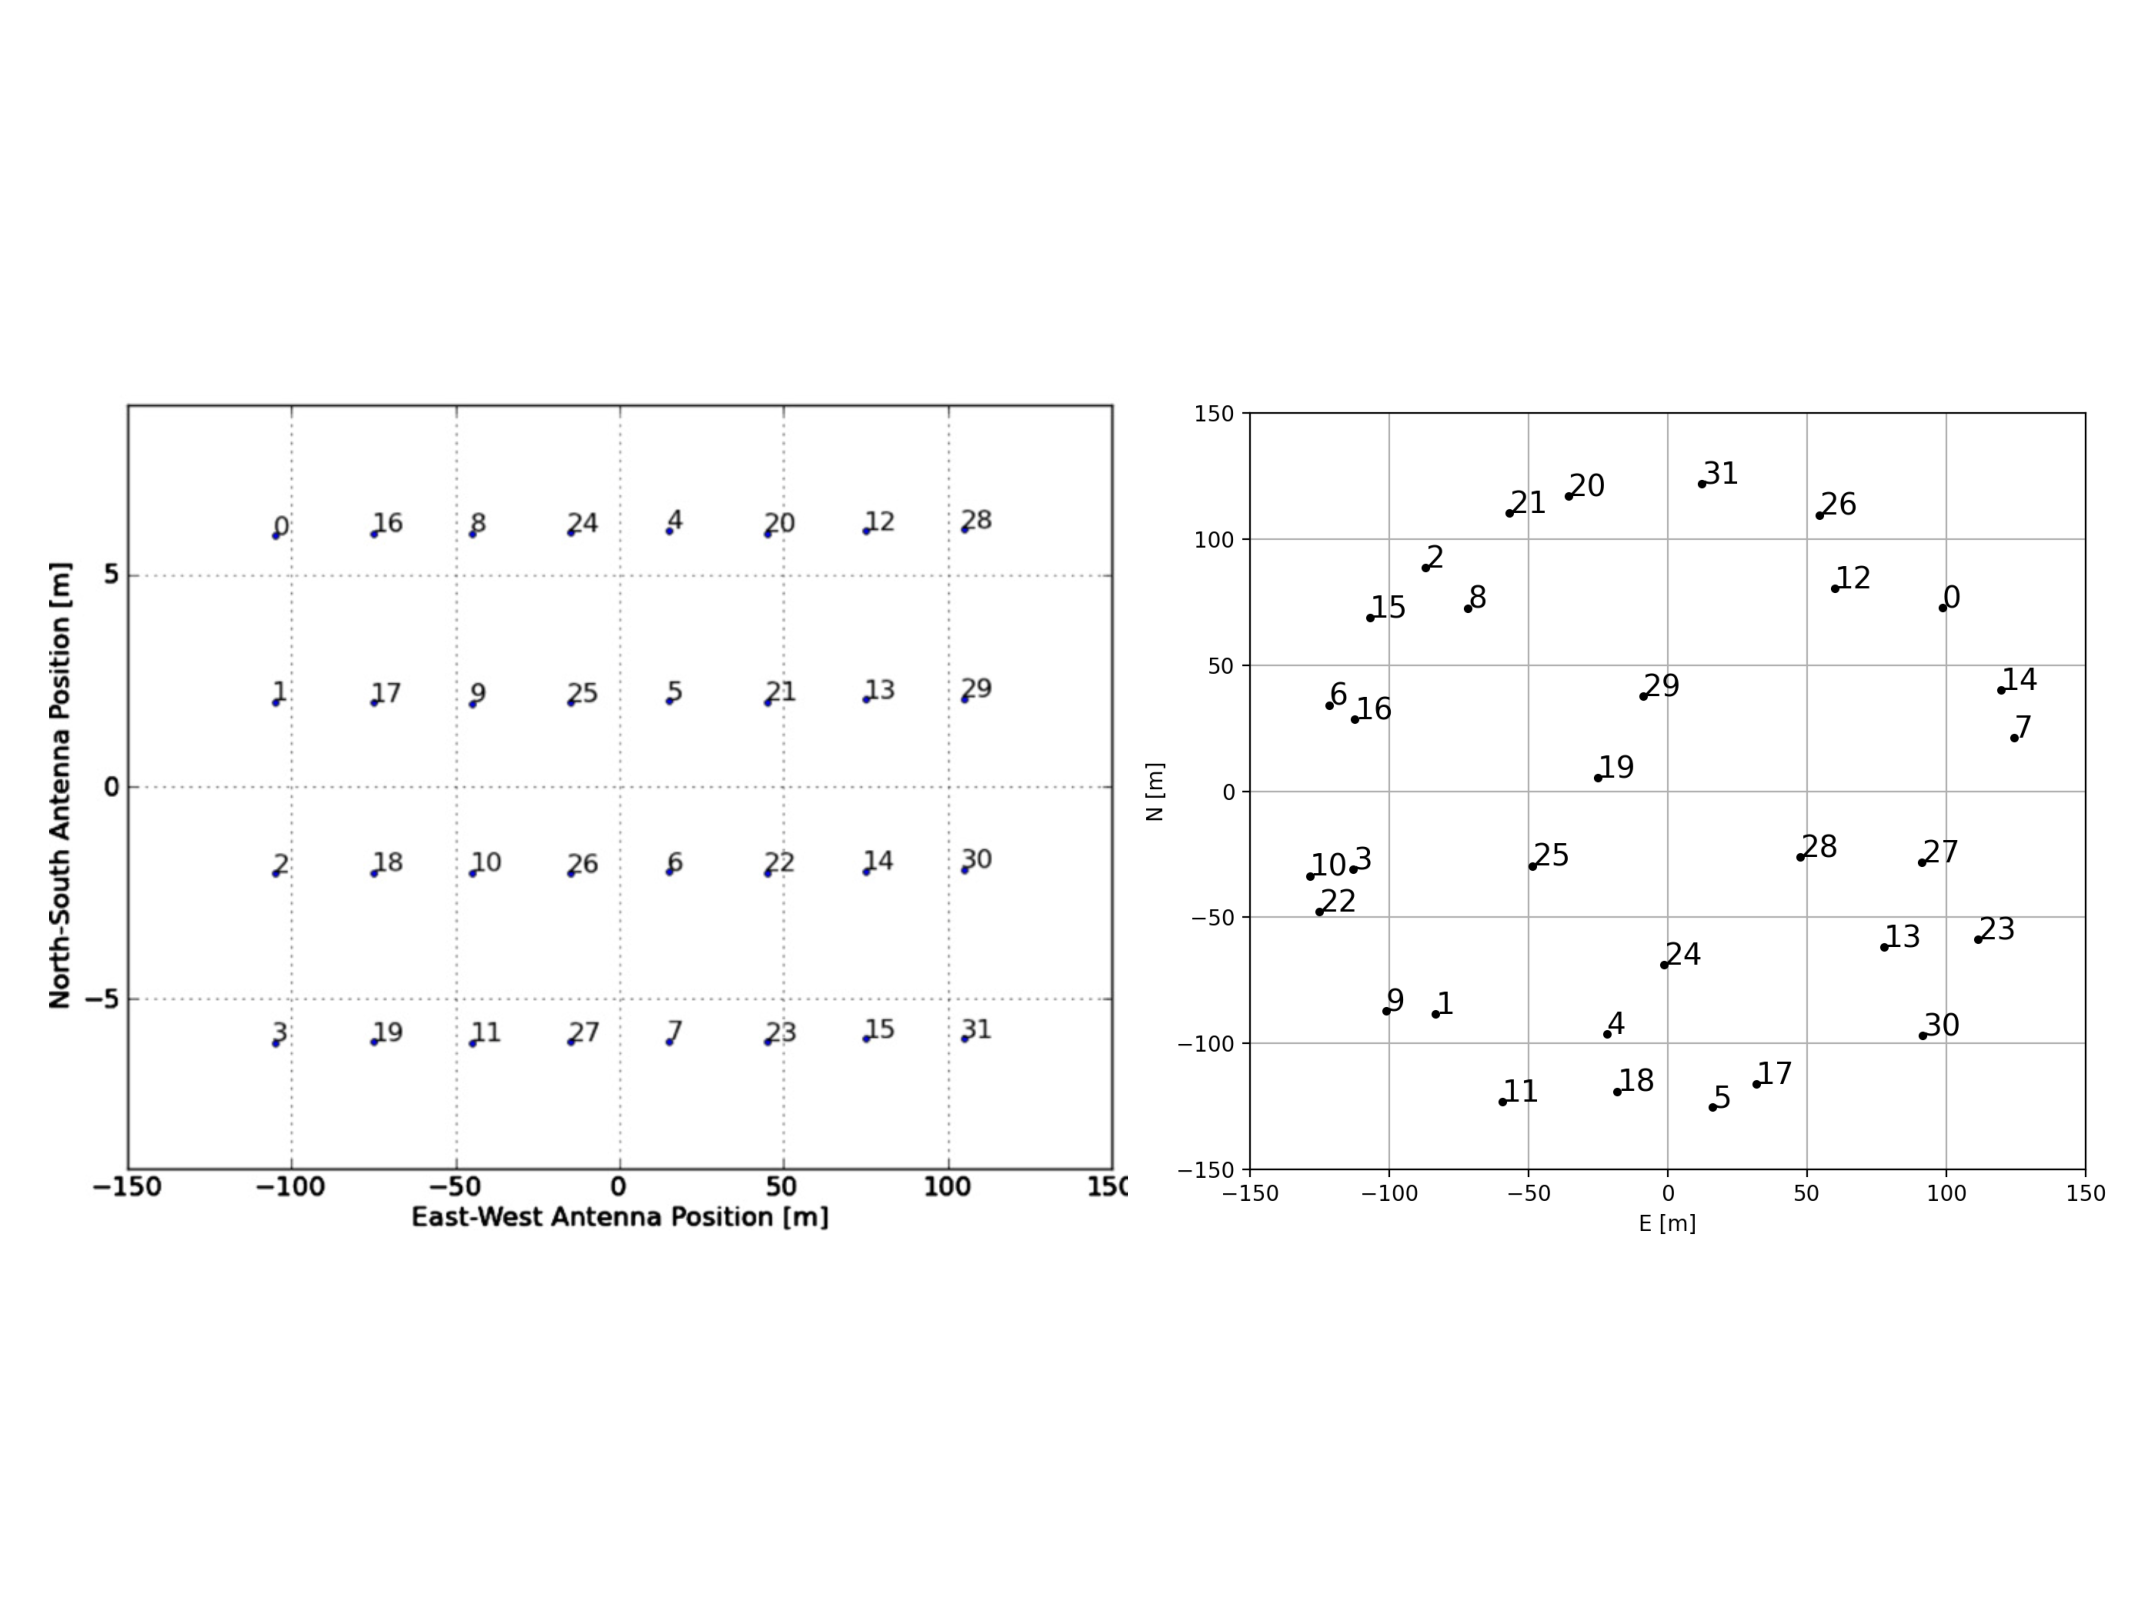
\includegraphics[width=0.9\textwidth]{chapters/instruments/figures/psa32_layouts.pdf}
\caption[The array layouts of the PAPER-32 element deployment in South Africa.]{The array layouts of the PAPER-32 element deployment in South Africa. \textit{Left}: The redundant grid. Four rows, with each element 30\,m from the next in the East-West direction, and closely-packed ($\sim$4\,m) in the North-South direction. Figure taken from \cite{Parsons.14}. \textit{Right}: The polarized imaging array. Elements were arranged in a pseudo-random scatter.}
\label{fig:instruments_psa32layout}
\end{figure}

\subsubsection{PAPER-64}

During the PAPER-32 EoR integration, there were actually 64 antennas present in the Karoo, South Africa. However, the correlator at that time could only process 64 voltage streams -- enough for 32 dual-polarization antennae. This is why 64 element single-instrument-polarization imaging results were published prior to any PAPER-32 studies \citep{Jacobs.13, Stefan.13}. EoR integrations in the 64 element redundant configuration were only possible after a new correlator was produced in 2012. Results from this array were published in \cite{Ali.15}, \cite{Pober.15}, Cheng et al. \textit{submitted} and Kolopanis et al. \textit{submitted}. The array layouts are shown in Figure~\ref{fig:instruments_psa64layout}.

\begin{figure}
\centering
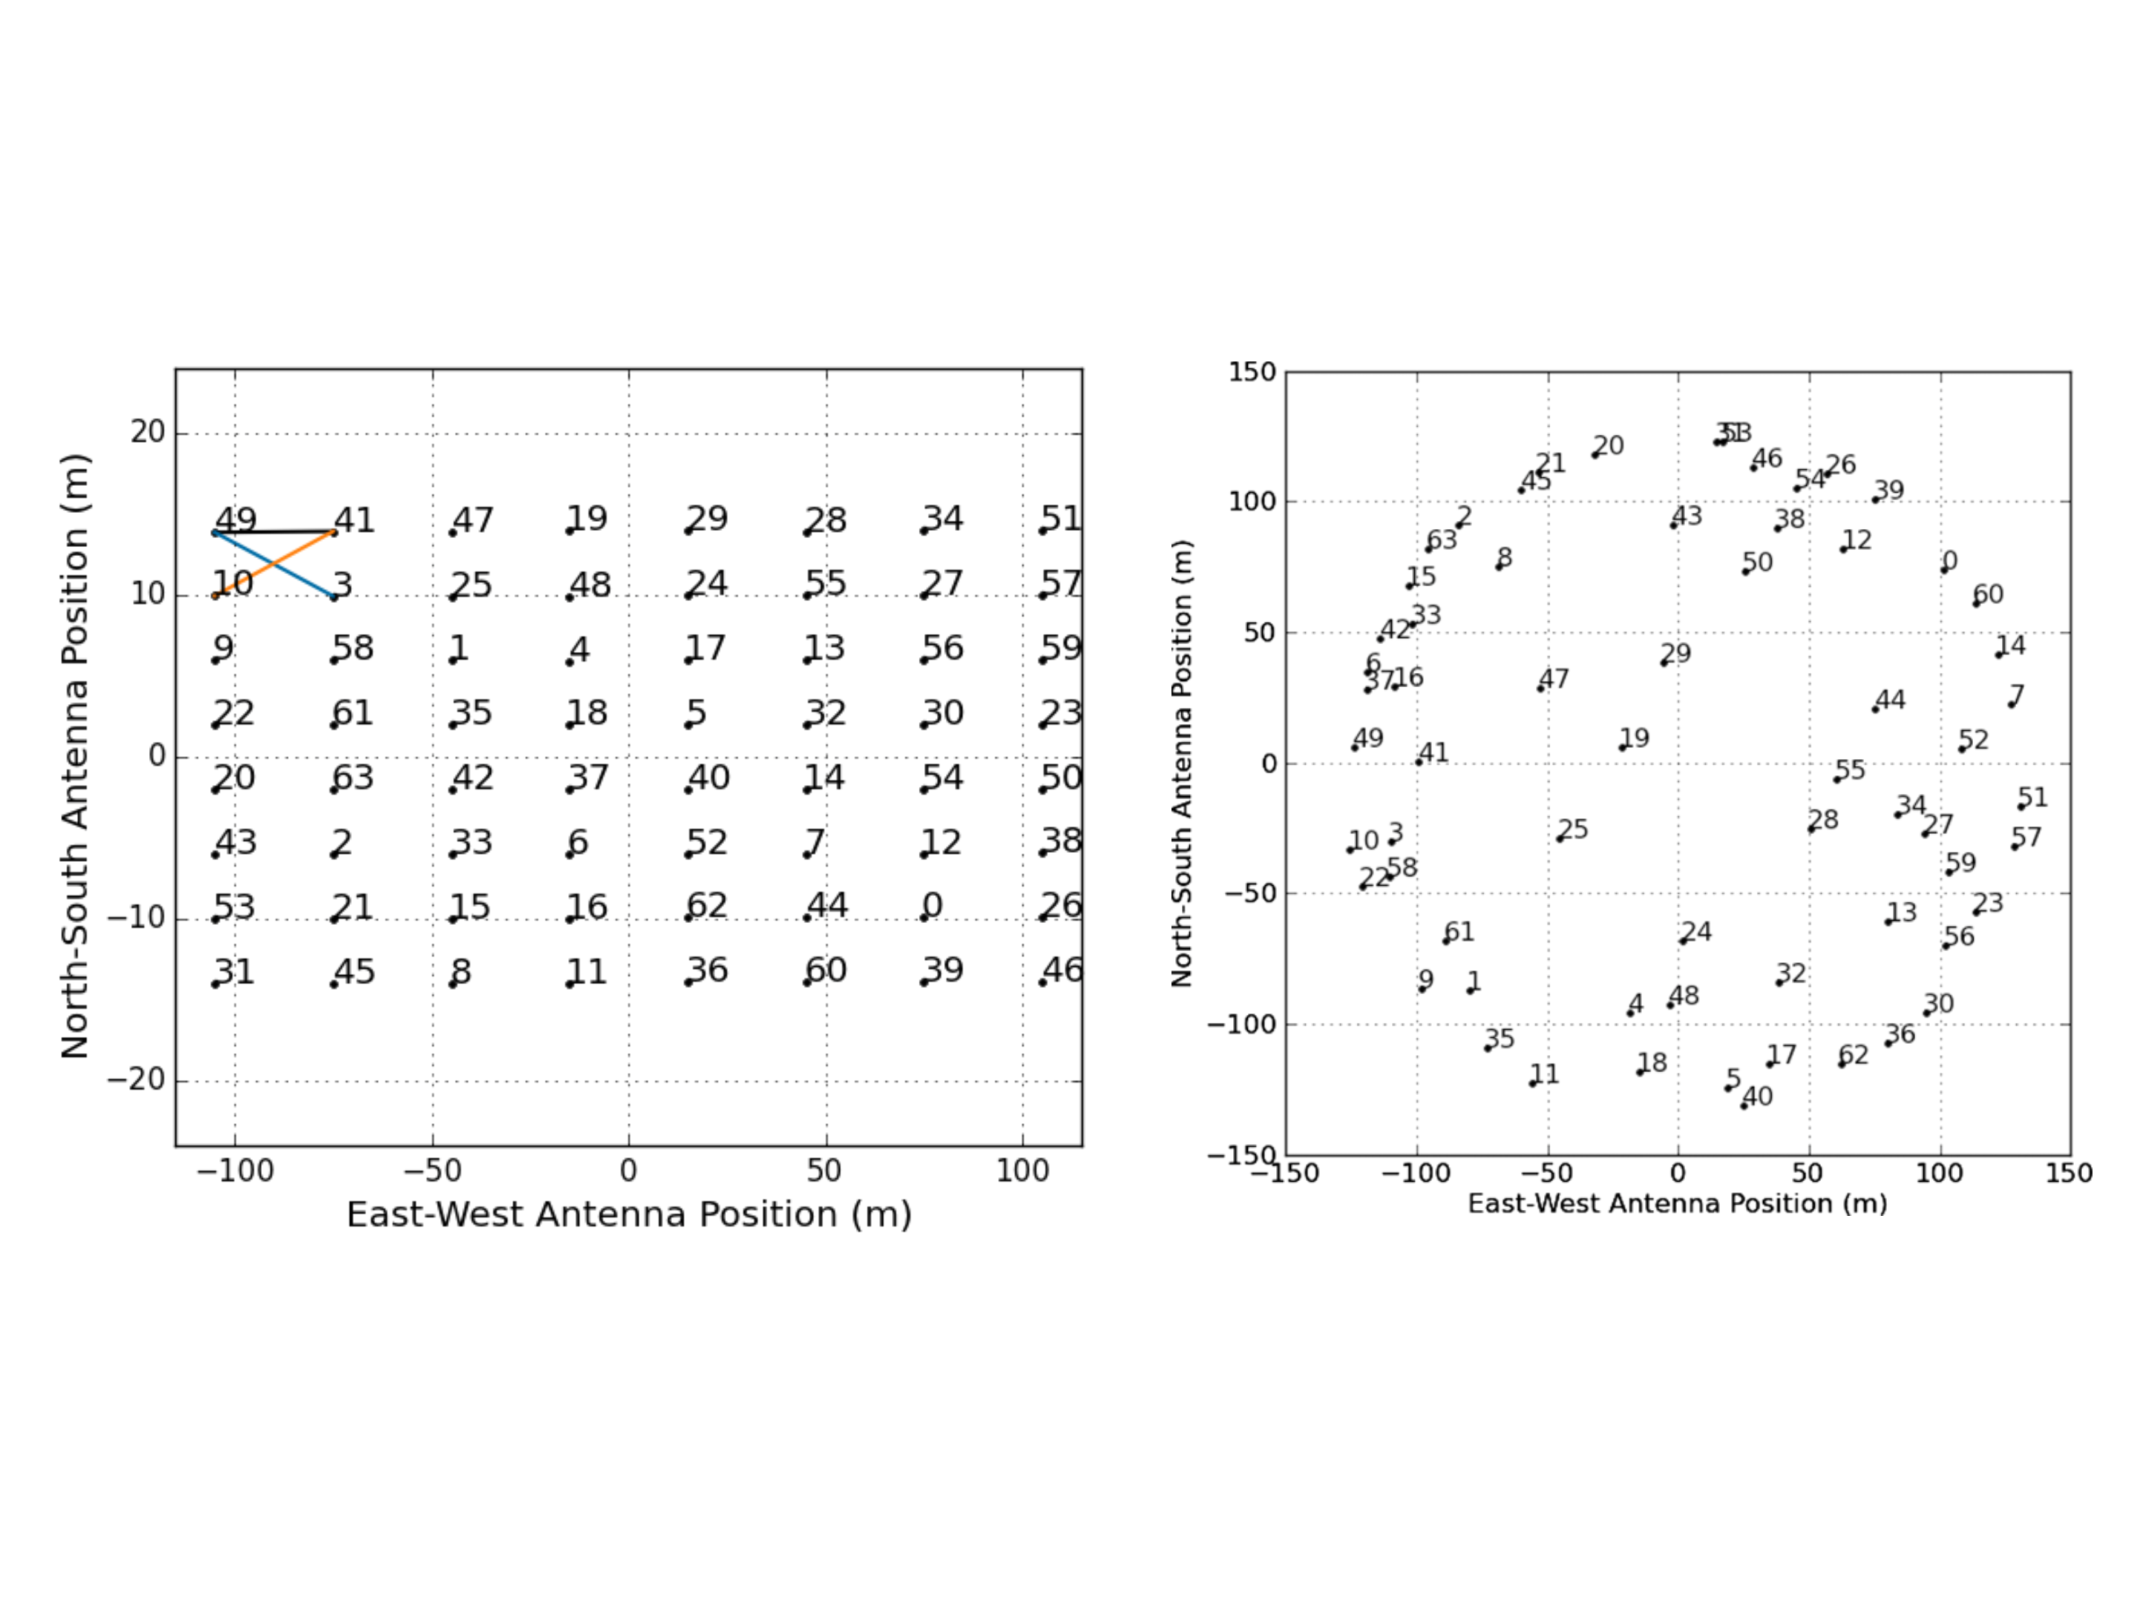
\includegraphics[width=0.9\textwidth]{chapters/instruments/figures/psa64_layouts.pdf}
\caption[The array layouts of the PAPER-64 deployment.]{The array layouts of the PAPER-64 deployment. \textit{Left}: The redundant grid, built-out from the PAPER-32 grid. Figure taken from \cite{Ali.15}, which highlights the baseline-types used for power spectrum measurements. \textit{Right}: the imaging array, used by \cite{Jacobs.13} to set an absolute flux scale for PAPER experiments. Figure taken from \cite{Jacobs.13}.}
\label{fig:instruments_psa64layout}
\end{figure}

\subsubsection{PAPER-128}

The culmination of the PAPER experiment was the 128 element deployment. There were two observing seasons recorded: November 2013 to March 2014, and July 2014 to January 2015. In this configuration, 112 antennas were laid-out in a redundant grid with 15\,m East-West spacings and 4\,m North-South spacings. The remaining 16 antennas were arranged in `out-rigger' and `in-rigger' positions to increase \textit{uv}-coverage and enable some level of imaging. Results from the first observing season of this array are presented in Chapters~\ref{chapter:data_prep_and_proc}, \ref{chapter:polcal} and \ref{chapter:eor_window_psa128}. The array layout is shown in Figure~\ref{fig:instruments_psa128}.

\begin{figure}
\centering
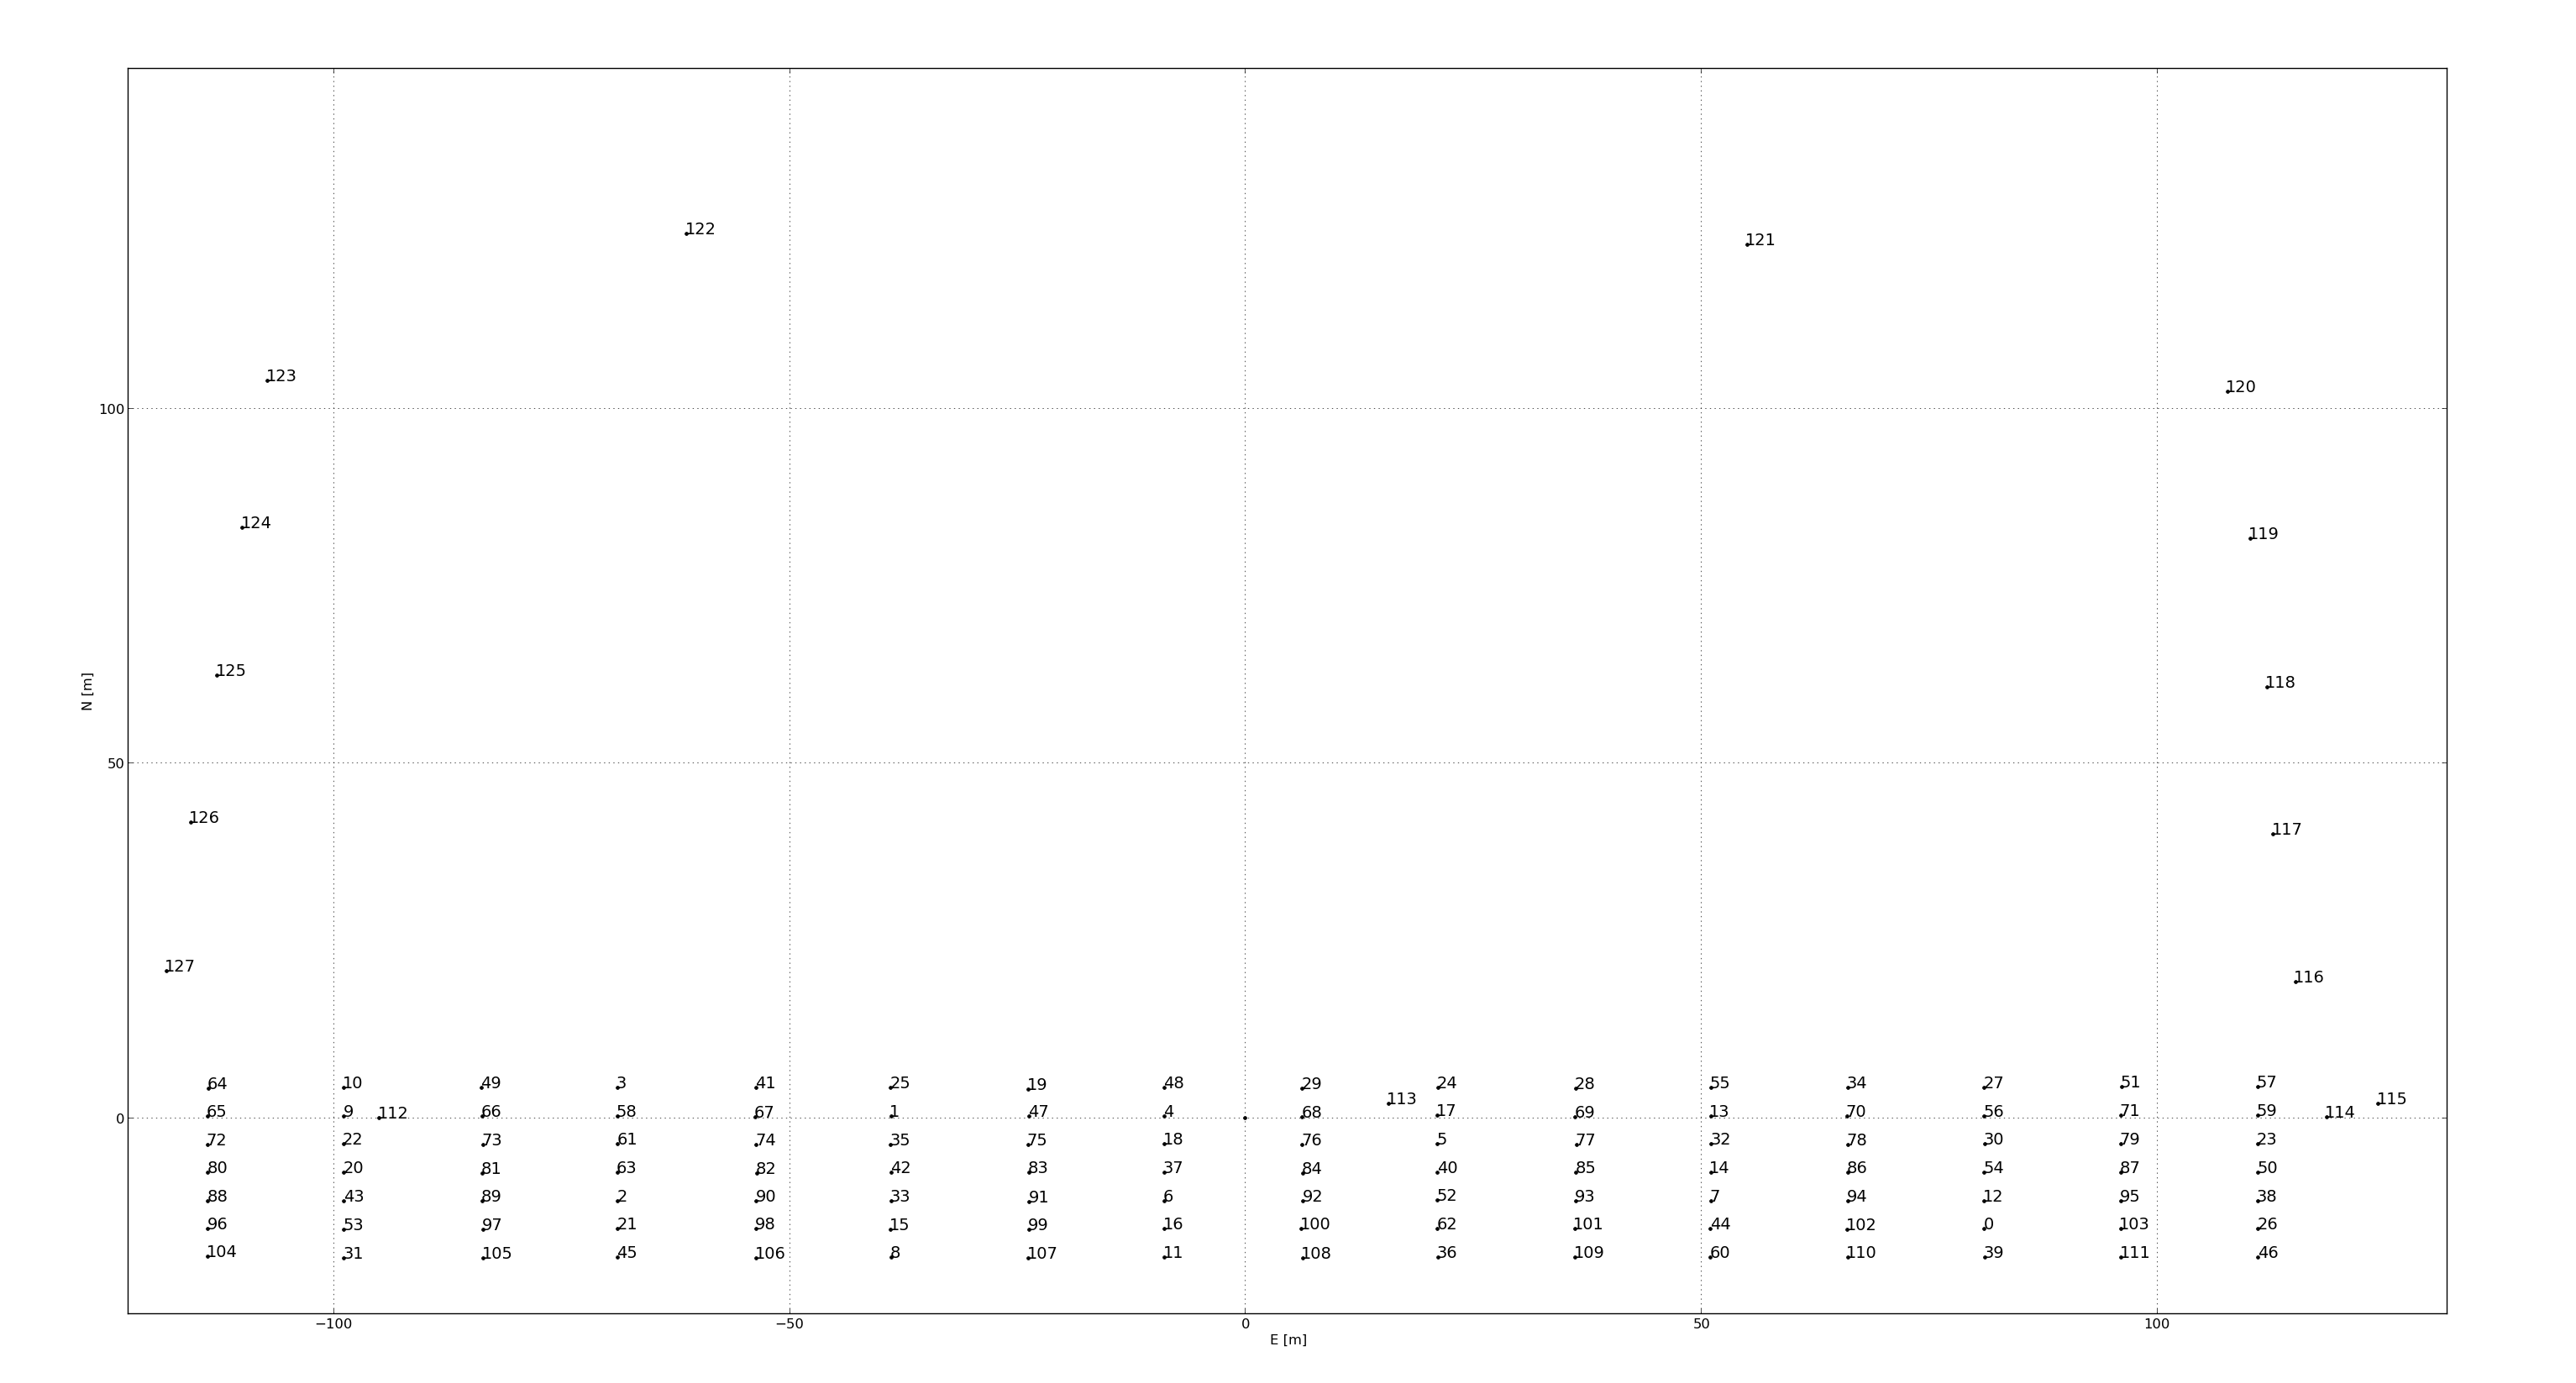
\includegraphics[width=0.9\textwidth]{chapters/instruments/figures/antlayout_psa128.png}
\caption[The PAPER-128 array layout.]{The PAPER-128 array layout. 112 antennas were laid-out in a redundant grid with 15\,m East-West spacings and 4\,m North-South spacings, and the remaining 16 antennas were arranged in `out-rigger' and `in-rigger' positions to increase \textit{uv}-coverage.}
\label{fig:instruments_psa128}
\end{figure}

\subsection{The Hydrogen Epoch of Reionization Array (HERA)}
\label{subsec:hera_instrument}

HERA was ranked as the ``top priority in the Radio, Millimeter, and Sub-millimeter category of recommended new facilities for mid-scale funding'' by the National Research Council Decadal Survey in astronomy and astrophysics \citep{Astro2010}. It brought together the largely US-based experts working on PAPER and the MWA to construct a new low-frequency array on the PAPER site in South Africa. The array, comprised of 14\,m diameter dishes, was designed to be build-out in stages of close-packed hexagons of increasing size. For a full description of the instrument, refer to \cite{deBoer.17}.

The design of the HERA dish, feed, antenna layout and signal chain are intimately related to lessons learned by the PAPER and MWA EoR teams about the nature of EoR measurements \citep[e.g.][]{Nithya.15a}. One of the major considerations was how the instrument couples to the bright foregrounds, and how to control that coupling -- the paradigm of the ``wedge'' and the ``EoR Window'', which are discussed in detail in Chapter~\ref{chapter:eor_window_theory}. Measurements based on prototype feeds were presented in \cite[][Patra et al. \textit{submitted}]{Ewall-Wice.16.HERA_Dish, Neben.16}.

HERA is a staged experiment, building-out in close-packed hexagons from a 19 element commissioning array, to 37, 127, 240 and finally 350 elements (320 in a dense, fractured core and 30 out-riggers, see \citealt{Dillon.16} for more detail). Figure~\ref{fig:instruments_hera_layout} shows a rendering of the core alongside an image of the HERA-19 commissioning array.

\begin{figure}
\centering
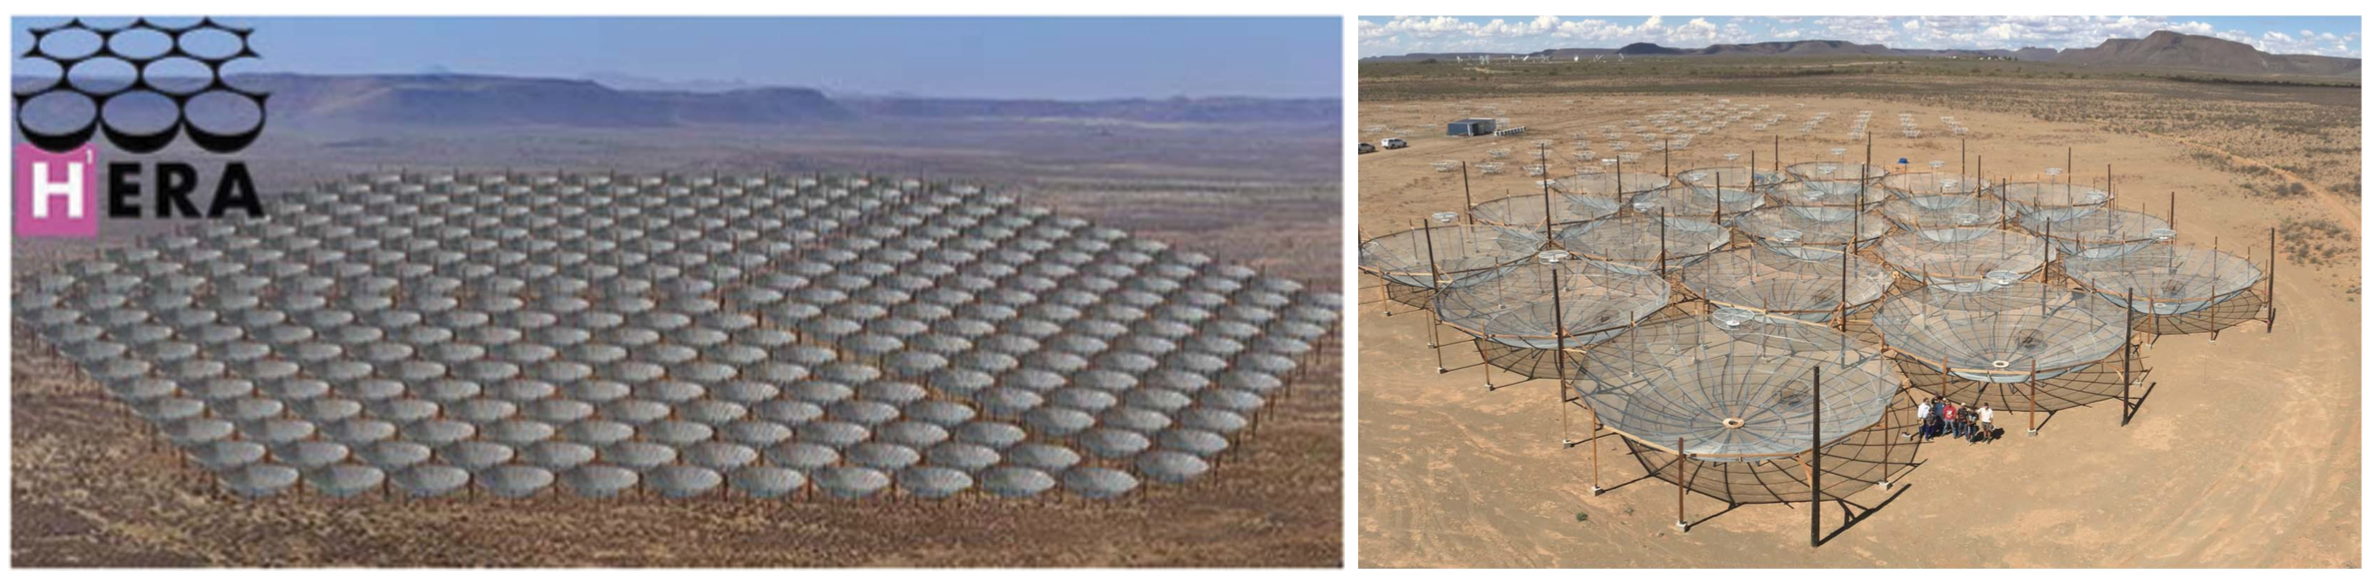
\includegraphics[width=0.9\textwidth]{chapters/instruments/figures/HERAlayout_deBoer.png}
\caption[Future vision and physical commissioning HERA layout.]{\textit{Left}: a rendering of the 320 element HERA core. \textit{Right}: the 19 element commissioning array (with the construction team). Leftover PAPER dipoles can also be seen in the background, forming three experimental arrays (described in Section~\ref{subsubsec:instruments_hera19}). Figure taken from \cite{deBoer.17}.}
\label{fig:instruments_hera_layout}
\end{figure}

\subsubsection{HERA-19 Commissioning Array}
\label{subsubsec:instruments_hera19}

In October 2015 a HERA commissioning array was completed, connected to the PAPER-128 256-input correlator. This array comprised of four separate components: the first 19 HERA dishes in a close-packed hexagon (HERA-19), 19 PAPER dipoles at the central locations of a hexagon of future HERA dishes (the ``PAPER-Hex''), 40 PAPER dipoles in a redundant grid where every-other dipole was rotated 45$^{\circ}$ (to experiment with different polarization bases; ``PAPER Pol''), and the remaining inputs filled with PAPER dipoles arranged in a pseudo-random scatter for imaging (``PAPER-Img''). Studies with this array are presented in Chapter~\ref{chapter:data_prep_and_proc} and \ref{chapter:eor_window_HERA}. A diagram of the commissioning setup is shown in Figure~\ref{fig:instruments_hera19_layout}.

\begin{figure}
\centering
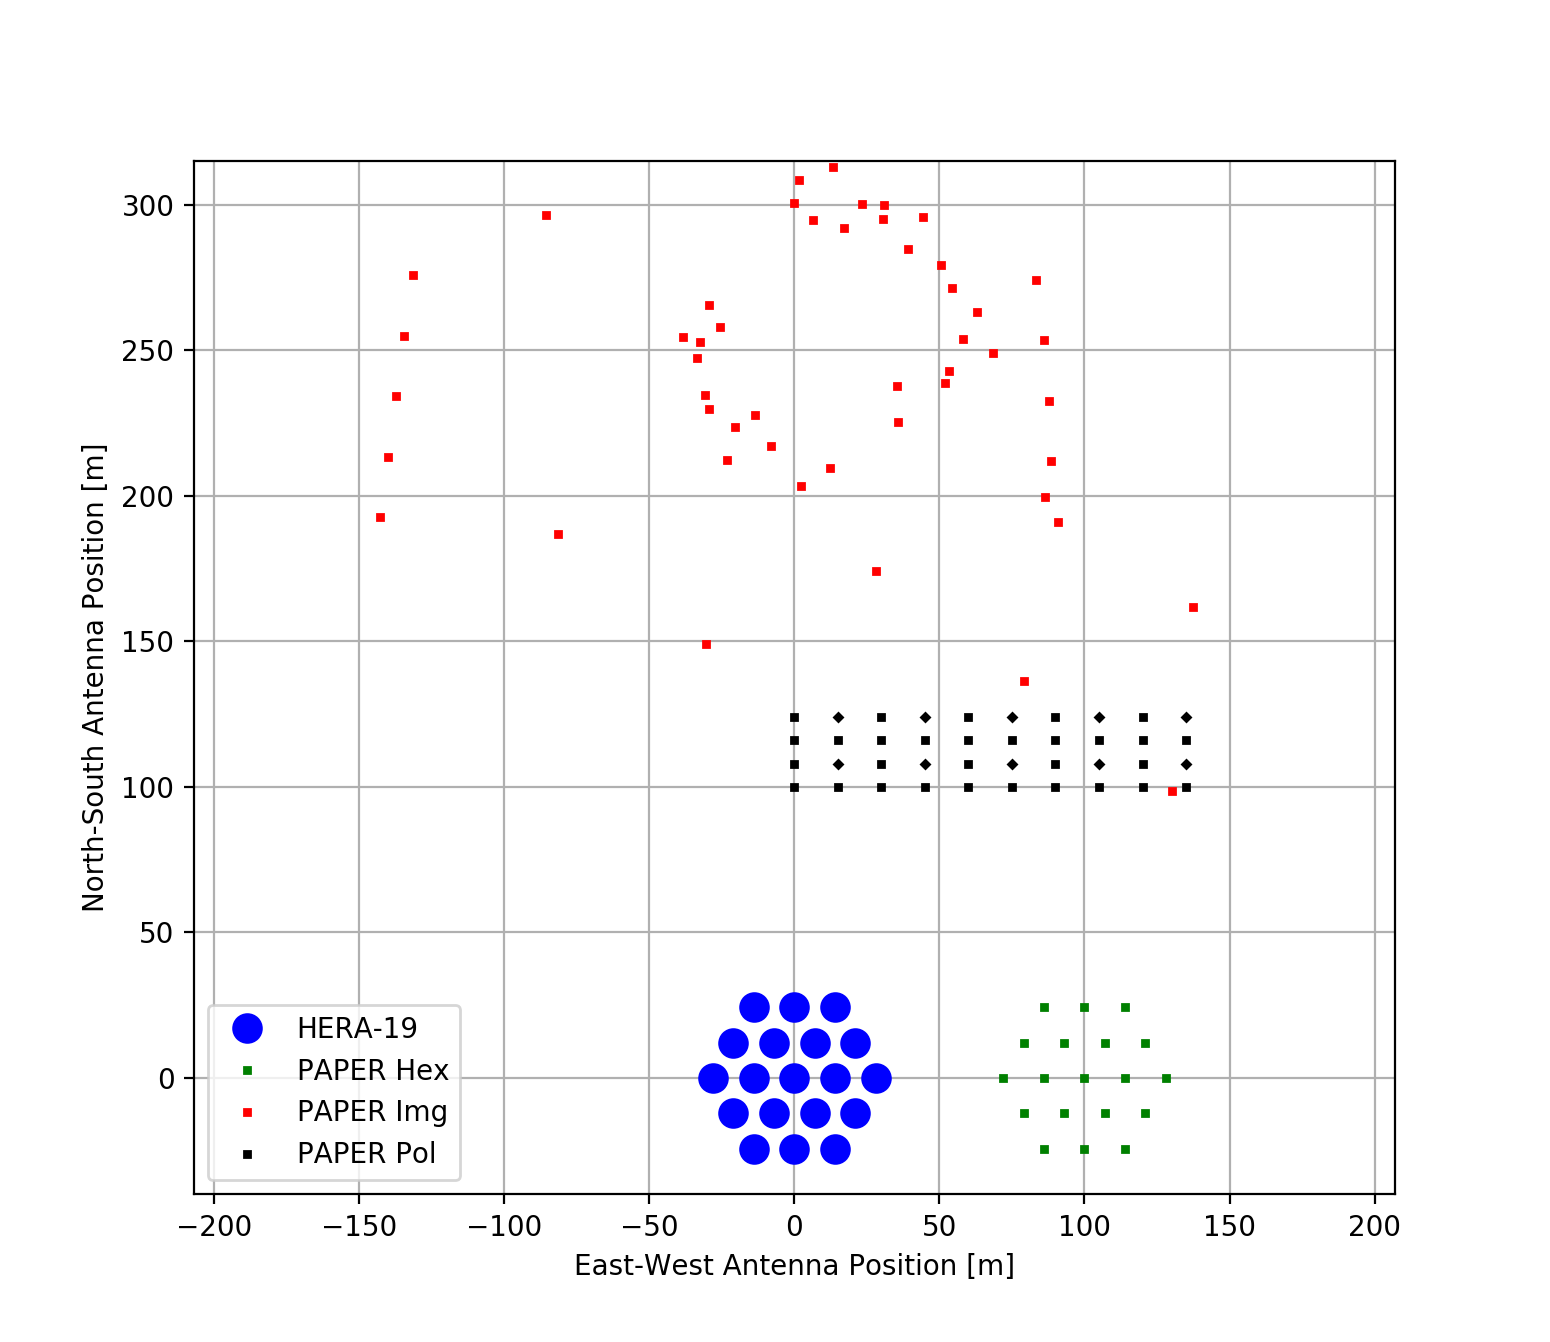
\includegraphics[width=0.9\textwidth]{chapters/instruments/figures/h19layout.png}
\caption{Positions of antennae in the HERA-19 Commissioning Array (including the experimental ``subarrays'').}
\label{fig:instruments_hera19_layout}
\end{figure}

\subsubsection{Future HERA Build-Outs}

Each HERA element is much more sensitive than a PAPER element, based purely on collecting area. Figure~\ref{fig:instruments_sensitivity} illustrates the varying sensitivities and collecting areas of different arrays and their elements, respectively. PAPER-128 was forecast to make marginal detections of the EoR power spectrum after $\sim$1000 hours of integration -- HERA-127 should be capable of characterizing the EoR power spectrum at high significance, and the full HERA-350 array will be an extremely powerful survey instrument \citep[e.g.][]{PoberMemo}. We present forecasts for this future instrument in Chapter~\ref{chapter:ksz_21cm}.

\begin{figure}
\centering
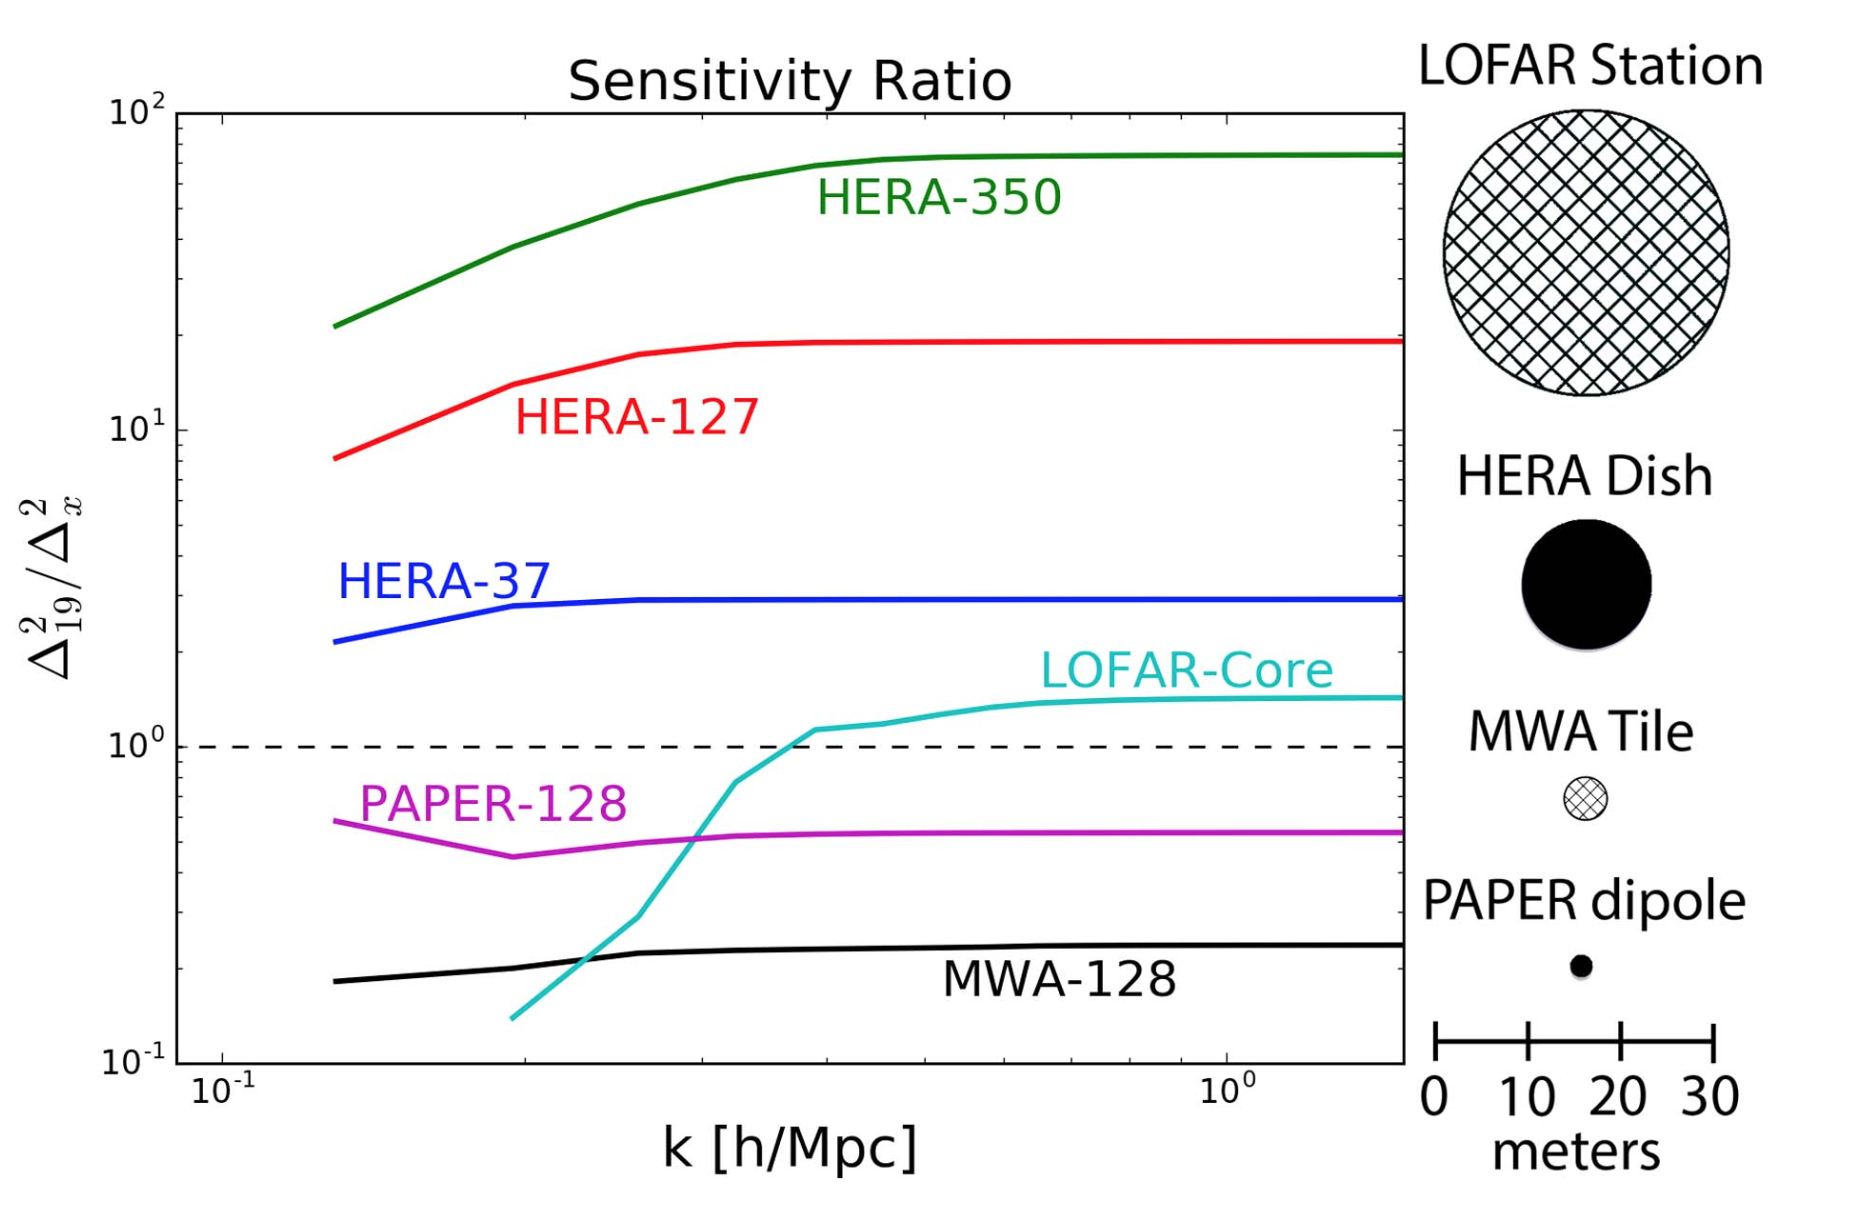
\includegraphics[width=0.9\textwidth]{chapters/instruments/figures/deBoer_sensitivities.png}
\caption[Array sensitivity as a function of \textit{k}-mode relative to HERA-19]{Instantaneous array Sensitivities as a function of \textit{k}-mode (e.g. Chapter~\ref{chapter:eor_window_theory}) relative to HERA-19. Differing element collecting areas are shown on the right. Taken from \cite{deBoer.17}.}
\label{fig:instruments_sensitivity}
\end{figure}

\section{Other current and future interferometers}
\label{sec:not_used_in_this_work}

PAPER and HERA were not the only instruments researching the EoR and how to detect it. Several low-frequency interferometers around the world are contributing to the understanding of the EoR and the difficulties of observing it. Below I briefly describe a few of the leaders of the field -- but it is not an exhaustive list.

\subsection{The Low Frequency Array (LOFAR)}

The LOw Frequency ARray (LOFAR) is an interferometer made-up of ``stations'', the core of which are arranged in a random scatter near Exloo in the Netherlands \citep{vanHaarlem.13}. LOFAR baselines extend across Europe with stations in Ireland, Sweden, Germany, Poland and other locations. These extremely long baselines can provide LOFAR with exquisite imaging capabilities. 

LOFAR has detected diffuse, linear polarization structures that may be related to the Milky Way's magnetic field and interstellar medium \citep{Jelic.15}. \cite{Patil.17} presented deep limits on the EoR power spectrum from one night of LOFAR data (also see \citealt{Yatawatta.13}). A series of publications has investigated polarization in Fourier space \citep{Jelic.14, Asad.15, Asad.16, Asad.17} -- results that we build upon and verify throughout this work.

\subsection{The Murchinson Widefield Array (MWA)}
\label{subsec:mwa_instrument}

The Murchinson Widefield Array (MWA), based in Murchison Radio-astronomy Observatory in Western Australia, is composed of 256 `tiles' of 16 feeds each. At the time of writing, 72 tiles are arranged in compact hexagonal configurations in an effort to increase EoR sensitivity while retaining imaging capabilities with the rest of the array. The most complete low-frequency catalog of the southern sky, GLEAM, was presented by \cite{Hurley-Walker.17}.

The MWA uses separate analysis pipelines for its EoR measurements \citep{Sullivan.12, Jacobs.16, Trott.16}, an concept that will be implemented on future HERA measurements. The MWA has detected polarized signal from diffuse Galactic emission \citep{Lenc.16, Lenc.17} and set deep limits on the EoR power spectrum \citep[e.g.][]{Dillon.14, Dillon.15}. Pioneering work on the ionosphere was accomplished using MWA data \citep[e.g.][]{Loi.15}, which we discuss in Chapter~\ref{chapter:ionosphere}.

\subsection{Square Kilometer Array -- Low band (SKA-Low)}
\label{subsec:skalow_instrument}

The Square Kilometer Array (SKA) will be built on two sites: the Karoo Radio Quiet Zone, currently occupied by HERA, will be the central location of the ``high--mid band'' (350 MHz -- 14 GHz; ``SKA-Mid'') observatory and the Murchinson Radio-astronomy Observatory, currently occupied by the MWA, will be the central location of the ``low band'' observatory (50 -- 350 MHz; ``SKA-Low'').

SKA-Low will consist of over 100,000 receiving elements in an imaging configuration. It will be the most powerful low-frequency radio telescope ever created, and be used not only for EoR science but a host of low-frequency science objectives \citep[e.g.][]{SKABook, Schilizzi.07, Dewdney.09}. Learning from the work of EoR teams working on PAPER, HERA, MWA, LOFAR and other instruments will be crucial to the success of SKA-Low's EoR science goals.
